\documentclass[10pt]{beamer}
\usepackage{amsmath}
\usepackage{mathtools}
\usepackage{multimedia}
\usepackage{hyperref}


\usefonttheme{professionalfonts} % using non standard fonts for beamer
\usefonttheme{serif} % default family is serif
%\documentclass[12pt]{beamerthemeSam.sty}
\usepackage{epsf}
%\usepackage{pstricks}
%\usepackage[orientation=portrait,size=A4]{beamerposter}
\geometry{paperwidth=160mm,paperheight=120mm}
%DT favorite definitions
\def\LL{\left\langle}	% left angle bracket
\def\RR{\right\rangle}	% right angle bracket
\def\LP{\left(}		% left parenthesis
\def\RP{\right)}	% right parenthesis
\def\LB{\left\{}	% left curly bracket
\def\RB{\right\}}	% right curly bracket
\def\PAR#1#2{ {{\partial #1}\over{\partial #2}} }
\def\PARTWO#1#2{ {{\partial^2 #1}\over{\partial #2}^2} }
\def\PARTWOMIX#1#2#3{ {{\partial^2 #1}\over{\partial #2 \partial #3}} }

\def\rightpartial{{\overrightarrow\partial}}
\def\leftpartial{{\overleftarrow\partial}}
\def\diffpartial{\buildrel\leftrightarrow\over\partial}

\def\BC{\begin{center}}
\def\EC{\end{center}}
\def\BN{\begin{enumerate}}
\def\EN{\end{enumerate}}
\def\BI{\begin{itemize}}
\def\EI{\end{itemize}}
\def\BE{\begin{displaymath}}
\def\EE{\end{displaymath}}
\def\BEA{\begin{eqnarray*}}
\def\EEA{\end{eqnarray*}}
\def\BNEA{\begin{eqnarray}}
\def\ENEA{\end{eqnarray}}
\def\EL{\nonumber\\}

\def\BS{\bigskip}
\newcommand{\etal}{{\it et al.}}
\newcommand{\gbeta}{6/g^2}
\newcommand{\la}[1]{\label{#1}}
\newcommand{\ie}{{\em i.e.\ }}
\newcommand{\eg}{{\em e.\,g.\ }}
\newcommand{\cf}{cf.\ }
\newcommand{\etc}{etc.\ }
\newcommand{\atantwo}{{\rm atan2}}
\newcommand{\Tr}{{\rm Tr}}
\newcommand{\dt}{\Delta t}
\newcommand{\op}{{\cal O}}
\newcommand{\msbar}{{\overline{\rm MS}}}
\def\chpt{\raise0.4ex\hbox{$\chi$}PT}
\def\schpt{S\raise0.4ex\hbox{$\chi$}PT}
\def\MeV{{\rm Me\!V}}
\def\GeV{{\rm Ge\!V}}

%AB: my color definitions
%\definecolor{mygarnet}{rgb}{0.445,0.184,0.215}
%\definecolor{mygold}{rgb}{0.848,0.848,0.098}
%\definecolor{myg2g}{rgb}{0.647,0.316,0.157}
\definecolor{A}{rgb}{1.0,0.3,0.3}
\definecolor{B}{rgb}{0.0,1.0,0.0}
\definecolor{C}{rgb}{1.0,1.0,0.0}
\definecolor{D}{rgb}{0.5,0.5,1.0}
\definecolor{E}{rgb}{0.7,0.7,0.7}
\definecolor{abtitlecolor}{rgb}{1.0,1.0,1.0}
\definecolor{absecondarycolor}{rgb}{0.0,0.416,0.804}
\definecolor{abprimarycolor}{rgb}{1.0,0.686,0.0}
\definecolor{Red}           {rgb}{1,0.4,0.4}
\definecolor{Yellow}           {rgb}{1,1,0.0}
\definecolor{Grey}          {cmyk}{.7,.7,.7,0}
\definecolor{Blue}          {cmyk}{1,1,0,0}
\definecolor{Green}         {cmyk}{1,0,1,0}
\definecolor{Brown}         {cmyk}{0,0.81,1,0.60}
\definecolor{Silver}        {rgb}{0.95,0.9,1.0}
\definecolor{Sky}           {rgb}{0.07,0.0,0.2}
\definecolor{Darkbrown}     {rgb}{0.4,0.3,0.2}
\definecolor{40Gray}        {rgb}{0.4,0.4,0.5}
\usetheme{Madrid}


\setbeamercolor{normal text}{fg=Silver,bg=Sky}

%AB: redefinition of beamer colors
%\setbeamercolor{palette tertiary}{fg=white,bg=mygarnet}
%\setbeamercolor{palette secondary}{fg=white,bg=myg2g}
%\setbeamercolor{palette primary}{fg=black,bg=mygold}
\setbeamercolor{title}{fg=abtitlecolor}
\setbeamercolor{frametitle}{fg=abtitlecolor}
\setbeamercolor{palette tertiary}{fg=white,bg=Darkbrown}
\setbeamercolor{palette secondary}{fg=white,bg=absecondarycolor}
\setbeamercolor{palette primary}{fg=white,bg=40Gray}
\setbeamercolor{structure}{fg=abtitlecolor}

\setbeamerfont{section in toc}{series=\bfseries}

%AB: remove navigation icons
\beamertemplatenavigationsymbolsempty
\title[From Ptolemy to Kepler]{
  \textbf {From Ptolemy to Kepler}}


\author [Astronomy 101]{Astronomy 101\\Syracuse University, Fall 2017\\Walter Freeman}

\date{\today}

\begin{document}



\frame{\titlepage}



\frame{\frametitle{\textbf{Announcements}}
\Large
\BI
\item Exams will be returned in lab next week
\item After lab, you'll know your grade
\item Scores will be posted on Blackboard as soon as they are scanned
\item {\bf Doublecheck your score} on Blackboard in case something went wrong
\BI
\item If you don't have a score or have a zero, you messed up your SUID -- don't panic, we'll fix it
\EI
\item If there is an error, write your lab TA and cc: me
\item{First paper due Monday 5PM}
\item{Take-home lab posted; due early December}
\EI
}

\frame{\frametitle{\textbf{Writing assignment}}
\Large \BC For those who missed it, the first paper is due next Monday.\EC

\BI
\item Potential for significant extra credit
\item Some special assignments for particular calendars; read the whole thing
\pause
\item Creativity is good -- there are lots of things you can write about besides
the ones I've used as examples
\EI

\BS
\BS

\BC To turn in your paper:\EC
\BI
\item Email a copy to {\tt suast101projects@gmail.com} by Monday at 5PM
\item Place a physical copy in your TA's mailbox by Monday at 5PM
\pause
\item If you will be gone Monday, get your TA's permission to turn it in late; this is fine, as long as the email is on time
\EI


}

\frame{\frametitle{\textbf{After class today:}}
\Large
There may or may not be a prelab next week. We are running behind preparing things because of a few urgent matters that came up.

\BS

If there is a prelab, it will be made available by the end of the day today and we'll email you.

\BS
\BS
\BS

There will be a warmup question posted by the end of the day today. We'll email out a reminder.

}




\frame{\frametitle{\textbf{Where we've come from, and where we're going}}
\Large
\BC
We are now able to predict the motions of most of the stuff in the night sky:
\EC
\BI
\item the distant stars
\item the Sun
\item the Moon
\item {\bf not} the planets!
\EI
}

\frame{\frametitle{\textbf{A word on archaeoastronomy}}
\large
Most ancient cultures looked at the stars in their own way, inheriting and
modifying the astronomical perspective of their forebears.

\BS\BS\pause

Many of them were extremely clever in different ways, discovering all sorts
of things about the stars before they were known to ``modern astronomy''.

\BI
\item Chinese astronomers kept meticulous records, and thanks to them we 
know details of the 1066 supernova
\item There are suggestions that the Australian Aboriginals knew about 
red-giant pulsation
\item Pacific Islanders' amazing talents at celestial navigation allowed them to travel long distances over open ocean
\EI

\BS

We'd be here for years if we looked at them all -- but you will have an 
opportunity to look at a few yourself in an upcoming paper!

\BS\BS\pause

Instead we're going to focus on the specific narrative that led, 
ultimately, to modern science -- from Alexandria (Egypt), through
the Islamic world, to Renaissance Europe.
}


\frame{\frametitle{\textbf{Where we've come from, and where we're going}}
\Large\BC We've casually mixed together ancient and modern perspectives:\EC

\begin{columns}
\column{0.5\textwidth}
\large
\BC The celestial sphere model \EC


\column{0.5\textwidth}
\large
\BC The heliocentric model \EC
\end{columns}

\begin{columns}
\column{0.5\textwidth}
\normalsize
\BC 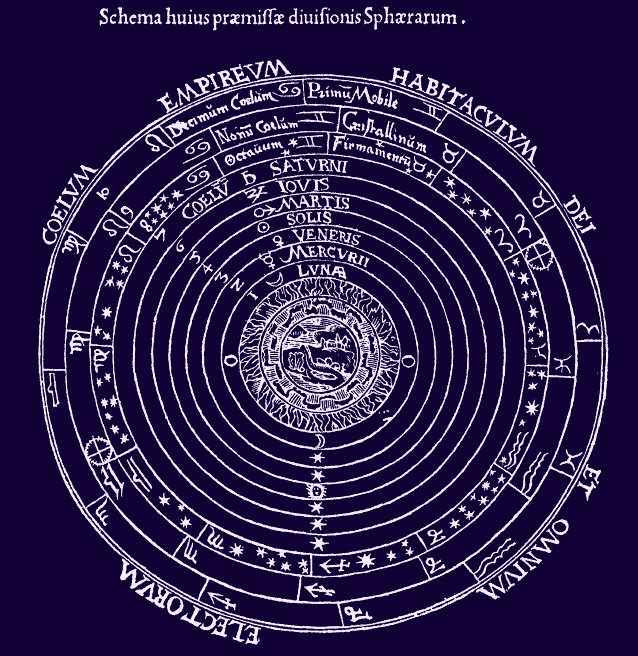
\includegraphics[width=0.6\textwidth]{sphere-medieval.png}\EC
\BI
\item{Heavenly bodies stuck to spheres}
\item{Spheres all turn around Earth}
\item{Planets, Sun, and Moon all have their own spheres}
\item{``Epicycles'' needed to get planets right}
\EI
\column{0.5\textwidth}
\normalsize
\BC 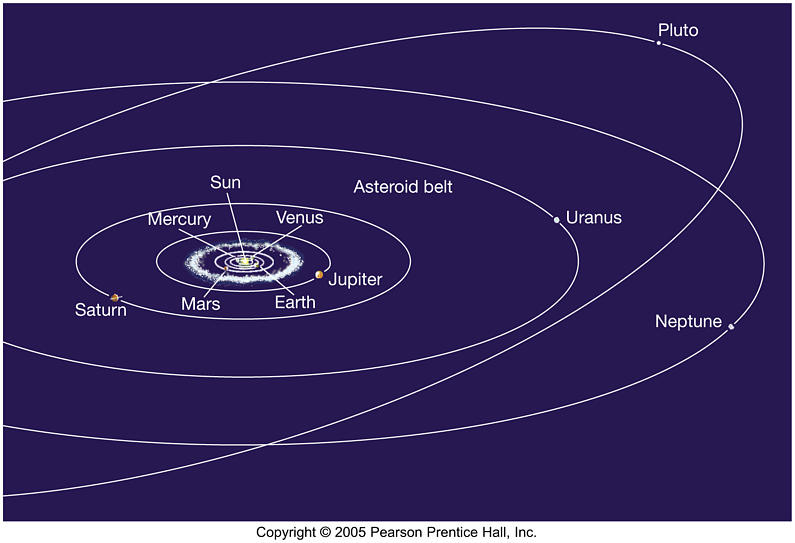
\includegraphics[width=0.7\textwidth]{ss-modern.jpg} \EC
\BI
\item{Earth is one of many planets, all orbiting the Sun}
\item{The Earth rotates on its axis}
\item{The stars are very far away and don't move}
\item{Modern perspective}
\EI
\end{columns}
}

\frame{\frametitle{\textbf{Where we've come from, and where we're going}}
\BC
\huge
How did this shift in perspective happen?

\bigskip
\bigskip
\bigskip
\bigskip

\pause

How was it part of the emergence of modern {\color{Green}science?}

\bigskip
\bigskip
\bigskip
\bigskip

\pause

... and what else did we learn about the sky in the process?
\EC
}


\frame{\frametitle{\textbf{Greek natural philosophy}}
\Large
The Greeks held philosophy in tremendous esteem. The branch of philosophy dedicated to explaining nature was {\it natural philosophy}.

\bigskip
\bigskip

\pause

Greek thinkers:

\BI
\item{saw the behavior of nature as {\it something we can understand}}
\pause
\item{proposed {\color{Red}natural}, not {\color{Red}supernatural}, causes for phenomena when possible}
\pause
\item{proposed {\color{Green}models} for things in nature}
\pause
\item{used {\color{Red}mathematics} in these models}
\pause
\item{recognized that any model had to agree with observation}
\EI
}

\frame{
\BC
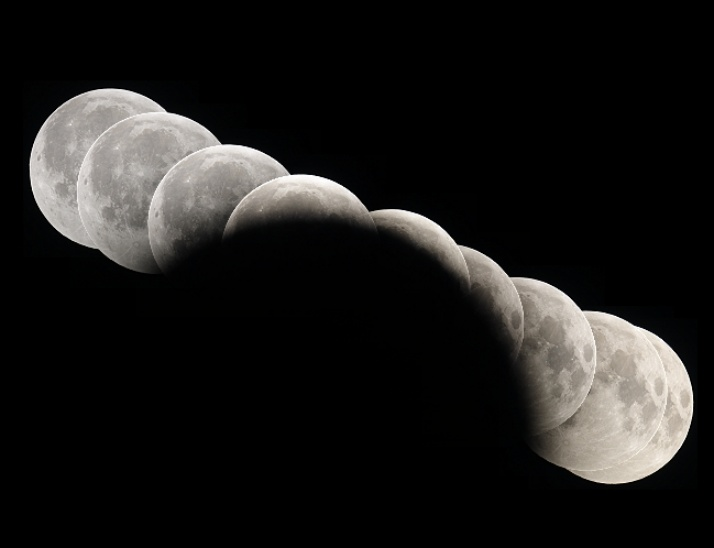
\includegraphics[width=0.6\textwidth]{lunar-eclipse-composite.jpg}
\Large
\bigskip

The Greeks realized that images of the Moon during an eclipse looked like this.
\EC
}

\frame{
\Huge
\BC
What might they learn from this?
\EC
\bigskip
\bigskip

\Large

\color{A}A: The Earth is round\\
\color{B}B: The Moon is about 400,000 km away\\
\color{C}C: The Moon is lit by the Sun, not from within\\
\color{D}D: The Earth orbits the Sun
}
\frame{\frametitle{\textbf{Greek natural philosophy}}
\Large
The Greeks held philosophy in tremendous esteem. The branch of philosophy dedicated to explaining nature was {\it natural philosophy}.

\bigskip
\bigskip


Greek thinkers:

\BI
\large
\item{saw the behavior of nature as {\it something we can understand}}
\item{proposed {\color{Green}models} for things in nature}
\item{used {\color{Red}mathematics} in these models}
\item{Believed in the transcendent Truth and Beauty of mathematical perfection}
\item{``Circles are the most perfect shape, thus things in the sky must go in circles''}
\item{\bf Increasingly saw astronomy as a separate discipline from natural philosophy (argh!)}
\EI
}



\frame{\frametitle{\textbf{Astronomy as separate from philosophy}}

\begin{columns}
\column{0.5\textwidth}
\BC\huge Natural philosophy\EC
\column{0.5\textwidth}
\BC\huge Greek astronomy\EC
\end{columns}

\begin{columns}
\column{0.5\textwidth}
\large
\BI
\item{Concerned with the fundamental Truth of things}
\item{Very concerned with logic, for instance}
\item{Saw the heavens as mostly outside their purview}
\item{Figuring out where the planets are is grunt work!}
\EI

\column{0.5\textwidth}
\large
\BI
\item{Concerned with {\it predicting} the motions of stars and planets}
\item{Not all that concerned with the {\it transcendent Truth} of their models}
\item{"... but do we get the right answer?"}
\item{Known mostly from Ptolemy's {\it Almagest}}
\EI
\end{columns}
}

\frame{\frametitle{\textbf{Observational facts at the time}}

\begin{columns}

\column{0.5\textwidth}

\large
Everything we already learned:

\BI
\item{Motion of the stars}
\item{Phases of the Moon}
\item{Seasons}
\item{Eclipses, etc.}
\EI
\column{0.5\textwidth}

No stellar parallax:

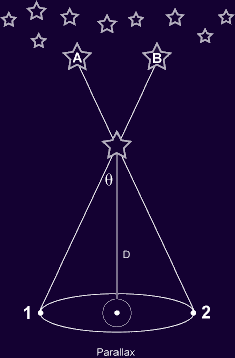
\includegraphics[width=0.6\textwidth]{parallax.png}
\bigskip
\bigskip

\end{columns}
}

\frame{\frametitle{\textbf{Observational facts at the time -- the hard one}}

\BC
\Large
Retrograde motion of planets:
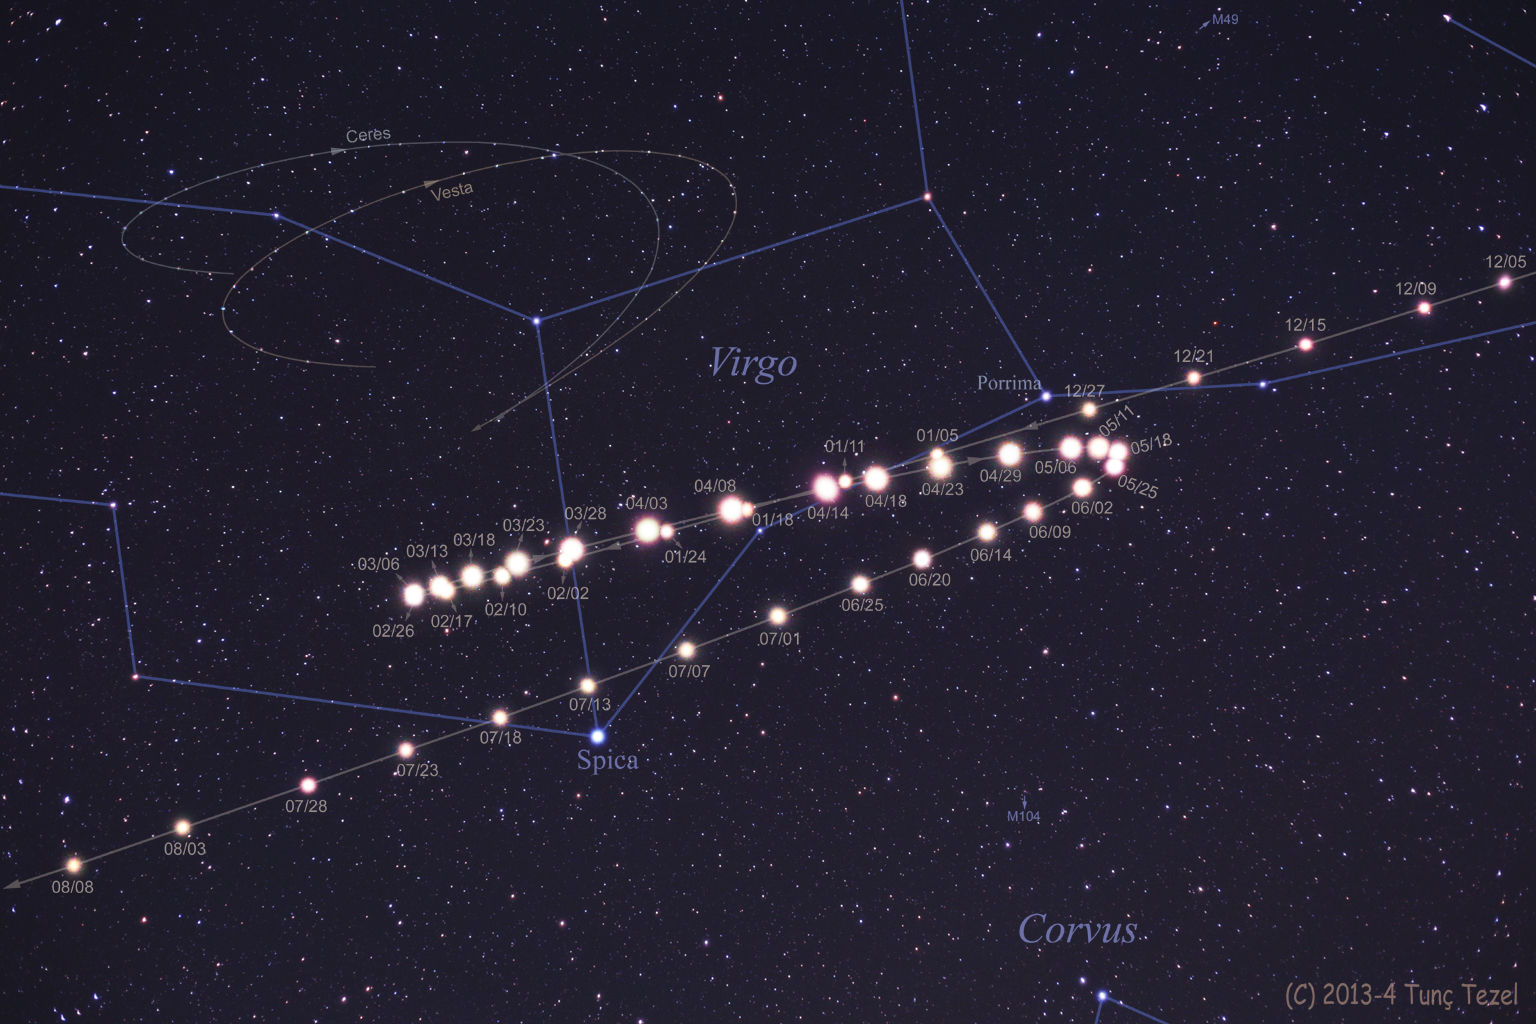
\includegraphics[width=0.85\textwidth]{retrograde.jpg}
\EC
}



\frame{\frametitle{\textbf{Ptolemy and his model}}
\large
Claudius Ptolemy lived in Alexandria, Egypt in the 2nd century CE.

\bigskip

This was a place and time where cultures met: Ancient Egypt, the Greek
tradition and culture, and the Roman Empire.

\bigskip
\bigskip
\bigskip

He was a nuts-and-bolts guy -- on the ``astronomy'' side of the philosophy/astronomy divide.

\bigskip
\bigskip
\bigskip

We know him mostly for his work {\it the Almagest}, a treatise on astronomy.

\pause

\bigskip
\bigskip
\bigskip

That doesn't sound Greek -- it's not. This name comes from Arabic, as do many others!
}

\frame{\frametitle{\textbf{Ptolemaic model}}
\large
Remember this? Ptolemy was the one who introduced it.

\bigskip

\BC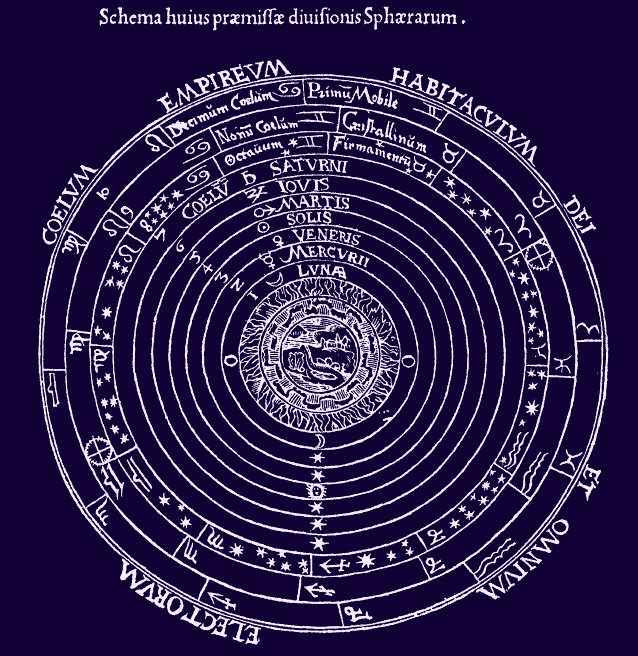
\includegraphics[width=0.4\textwidth]{sphere-medieval.png}\EC

\bigskip

\BI
\item{Everything is attached to crystal spheres which spin in a uniform, perfect way around the Earth...}
\pause
\item{... well, sort of: the Earth isn't {\it quite} at the center of the planet-spheres}
\item{... well, sort of: they don't turn {\it quite} uniformly, but with a fudge that keeps the perfection of ``circles''}
\EI

\bigskip

These modifications are necessary to get details of the motions of the planets right.

}

\frame{\frametitle{\textbf{Epicycles}}
\BC\Large
This still fails to reproduce retrograde motion. What's the solution? More circles!
\EC
\bigskip
\bigskip

\BC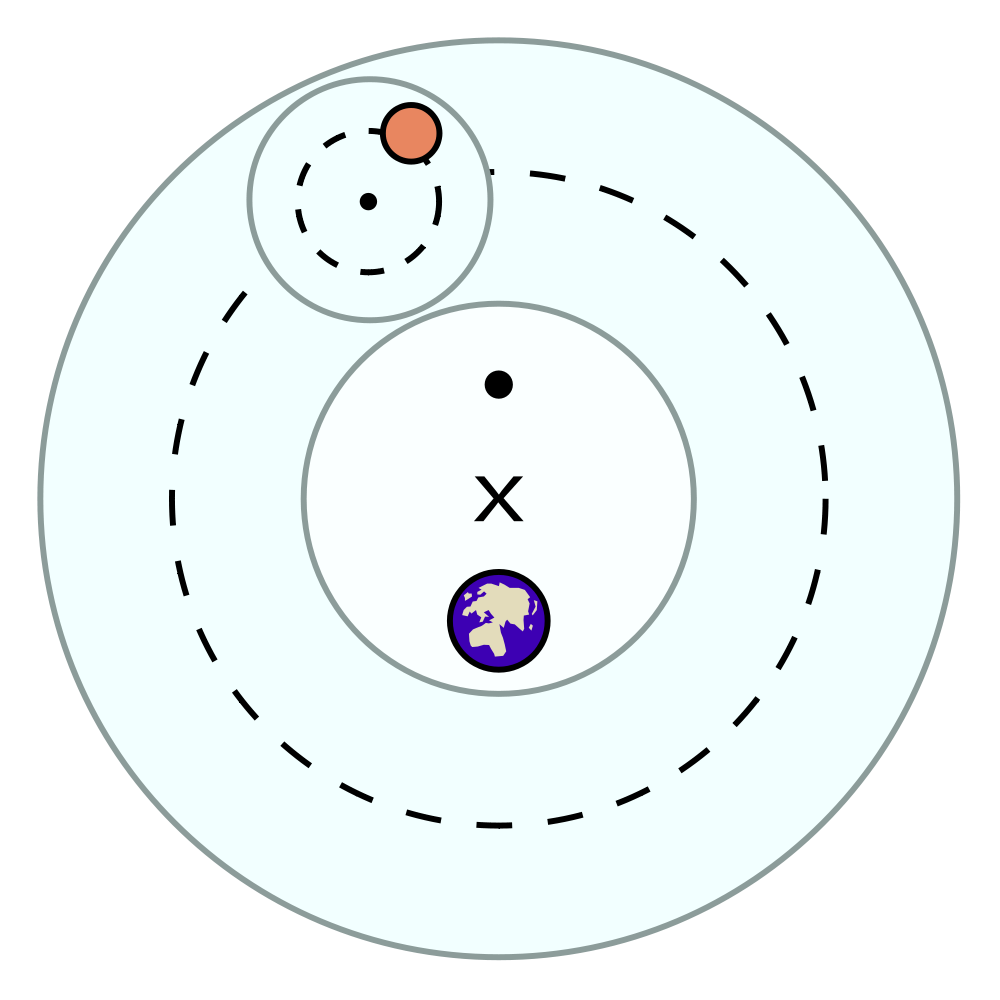
\includegraphics[width=0.3\textwidth]{epicycle1.png}\EC

\bigskip
\bigskip

These circles-on-circles are called ``epicycles''. The center of the epicycle rotates not-quite-uniformly about a point not-quite-at-Earth, and then
the planet rotates in a circle along the epicycle.

\pause
\bigskip
\bigskip

Confused? Let's watch this in action: \url{https://youtu.be/utH-GHH1FT8?t=64}
}

\frame{\frametitle{\textbf{The model in the Almagest}}
\Large
This model had a huge number of moving pieces: cycles on top of cycles, different centers and motion-fudges for each planet...

\bigskip
\bigskip
\bigskip

\pause

... but it WORKED. Ptolemy published tables in the {\it Almagest} that could be used to predict, with astonishing precision, where the planets would be -- even if he needed dozens of epicycles in total to do it.}


\frame{\frametitle{\textbf{What do you think about this?}}

\Large
\color{A}A: This is far too complicated to be Truth; the Universe shouldn't be this hard\\
\BS
\color{B}B: Some things are complicated; if this gets the right answer, then it is True\\
\BS
\color{C}C: Truth is overrated; what matters is whether a model is useful for what it was designed to do\\
\BS
\color{D}D: There is an abstract truth about nature, and a true model might predict other things we didn't expect\\\pause
\BS
\color{E}E: Epicycles are just alternative facts!
}



\frame{\frametitle{\textbf{From Egypt to Europe by way of the Islamic world}}
\Large
Alexandria in Egypt was the center of learning in the Western world ... until it wasn't.

\large

\bigskip
\bigskip

The great Library at Alexandria was burned (everyone blames everyone else for this), and Alexandria declined as a center of scholarship.

\bigskip
\bigskip

The Muslims studied the Greek writing, and accumulated a great deal of knowledge about the motions of the sky; they named many of the stars, refined
Ptolemy's model, 
and made enormous strides in {\it mathematics} (Arabic numerals, {\it al-jabr} (algebra), etc.)

\bigskip
\bigskip

}

\frame{\frametitle{\textbf{The state of Europe, pre-Renaissance}}
\Large
Europe didn't really have much of a natural-philosophic or scientific tradition from the fall of the Roman Empire to c. 1400.

\bigskip
\bigskip

Ptolemaic model was known, but mostly just applied (remember, this is ``astronomy'', not Real Philosophy)

\bigskip
\bigskip

\pause

``How many angels can dance on the head of a pin?'' (not quite)
}

\frame{\frametitle{\textbf{Copernicus (Polish/German, 1473-1543)}}
\Large

Ptolemy's model still worked -- {\it brilliantly}. It was only off by a few degrees in a thousand years.

\bigskip
\bigskip

People had started to be dissatisfied with the complexity of it. It just {\it felt} inelegant!

\bigskip
\bigskip

Enter Copernicus. He proposed that, instead, everything orbits the Sun in perfect circles.

\BI
\item{Ptolemy's model was {\it geocentric} -- the Earth is at the center}
\item{Copernicus' model was {\it heliocentric} -- the Sun is at the center}
\EI

\bigskip
\bigskip

This allowed him to explain retrograde motion -- {\it without} epicycles! (This is next week's lab.)}


\frame{\frametitle{\textbf{The philosophy of Copernicanism}}
\BC
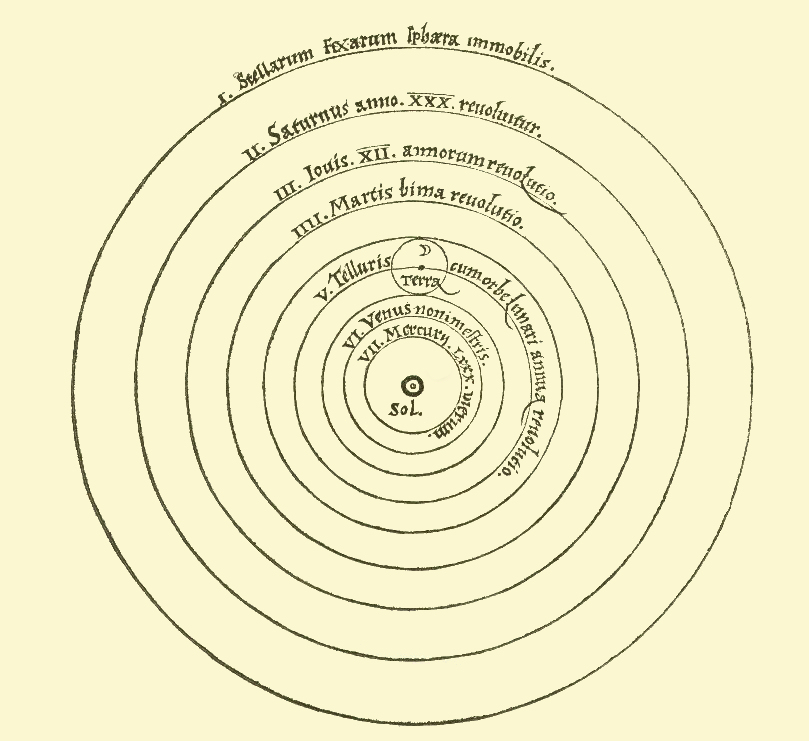
\includegraphics[width=0.5\textwidth]{copernican-model.jpg}
\EC

\Large
The publisher added a preface to his book, saying, essentially:

\bigskip

\BC \it
``This is unusual. But it is just mathematics; it should be judged on whether or not it makes accurate predictions; this is {\it separate} from whether it contains
actual philosophical truth!''

\EC

}


\frame{\frametitle{\textbf{The reality of Copernican heliocentrism}}
\Huge

\BC

How should we judge Copernicus' model?

\EC

\bigskip
\bigskip
\bigskip
\large
\color{A}A: Whether it is simpler than Ptolemy's, and still more or less predicts things well \\

\bigskip

\color{B}B: Whether it is more aesthetically pleasing -- more {\it elegant} -- and still more or less makes accurate predictions \\

\bigskip

\color{C}C: Forget simplicity and elegance -- are its predictions more precise? (Remember, Ptolemy's model was wrong by a degree after a thousand years) \\

\bigskip

\color{D}D: Whether it predicted anything {\it new} that hadn't been observed before  

}

\frame{\frametitle{\textbf{The reality of Copernican heliocentrism}}
\Huge

Whoops. 

\pause

\bigskip
\bigskip
\bigskip

\Large

Copernicus' model was actually {\it less precise} than Ptolemy's at predicting celestial motion. You could fix it up with epicycles, but not even all that well...

}


\frame{\frametitle{\textbf{Enter Galileo}}
\Large

Galileo Galilei, of northern Italy in the early 1600's, did a great many things. But, most important to us: he perfected the {\it telescope}, invented recently in the Netherlands.

\pause

\bigskip
\bigskip
\bigskip

He also pointed it at Jupiter, and saw this:

\url{https://www.youtube.com/watch?v=XpsQimYhNkA} (video from NASA)

\pause

\bigskip
\bigskip

{\bf There are things orbiting Jupiter!} These are the four largest moons of Jupiter, called the ``Galilean moons'' after their discoverer.

\BI
\item{If things orbit Jupiter, then not everything orbits the Earth! We are not the center of everything!}
\item{This was a huge shakeup -- to philosophy, and to {\it religion!}}
\EI
}

\frame{\frametitle{\textbf{The ``Galileo Affair''}}
\BI
\item{Galileo published what he saw with his telescope in 1610.}
\item{He argued that the moons of Jupiter, along with the phases of Venus, proved the Earth moved.}
\item{Now Galileo has left {\it astronomy} -- predicting things -- and entered philosophy!}
\pause
\item{Something else happened between Copernicus and Galileo: the Protestant Reformation and the Counter-Reformation!}
\item{This meant that the Church had gotten a bit touchy about theology and heresy.}
\pause
\item{In 1616 the Church declared heliocentrism heretical}
\item{In 1632 Galileo published a popular book, {\it Dialogue Concerning the Two Chief World Systems}, defending heliocentrism}\pause
\item{In 1633 the Inquisition declared him a heretic, banned all his books, and sentenced him to house arrest until he died in 1642.}
\pause
\item{The Church un-banned his books and heliocentrism in 1835.}
\EI
}




\frame{\frametitle{\textbf{Where we've come from, and where we're going}}
\Large

Galileo's work began a shift from {\it astronomy} to {\it astrophysics}.

\begin{columns}
\column{0.5\textwidth}
{\color{Red}\BC \huge (Ancient) Astronomy \EC}
\column{0.5\textwidth}
{\color{Red}\BC \huge Astrophysics \EC}
\end{columns}

\begin{columns}
\column{0.5\textwidth}
\large
\BI
\item{Predicts the motion of things}
\item{Not that concerned with their nature}
\item{An exercise in calculation}
\EI

\column{0.5\textwidth}
\large
\BI
\item{Concerned with understanding the {\it nature} of things in the sky}
\item{``What are they and by what rules do they operate?''}
\item{Predict their motion by understanding their nature}
\EI


\end{columns}

\bigskip

\BC
\huge
There's a reason you are taking this class in the physics building!
\EC
}

\frame{\frametitle{\textbf{... but it doesn't quite work!}}

\Large
For all of Galileo's ``proof'' that the Earth moves around the Sun, Ptolemy's model still made better predictions than Copernicus' model!

\bigskip
\bigskip
\bigskip
\pause

\huge What would be the best next step?

\bigskip
\bigskip
\bigskip

\large

\color{A}A: Doublecheck Copernicus' math, to see if his circles could be realigned to get better results\\ \bigskip 
\color{B}B: Make the most precise measurements of the planets that you can\\ \bigskip 
\color{C}C: Find other heliocentric models besides the one Copernicus had\\ \bigskip 
\color{D}D: Stick the Galilean moons around Jupiter in the Ptolemaic model and accept it as true \bigskip

}

\frame{\frametitle{\textbf{Three of these happened!}}

\Large
\BI
\item{Someone made impressively precise measurements of the motions of the planets}
\item{Someone doublechecked Copernicus' math:}
\BI
\item{... they found that a different arrangement of circles {\it almost} matched the data}
\item{... but it was off by one-eighth of a degree!}
\EI
\item{They found {\it another} heliocentric model, not using circles (!), that fit {\it perfectly}}
\pause
\item{Next time: this story, and a full transition to modern science}
\EI
}

\frame{\frametitle{\textbf{Summary}}
\BI
\item{Ancient Greeks separated philosophy from astronomy:}
\BI
\item{Philosophy: what is Truth?}
\item{Astronomy: how can I calculate when Venus will rise?}
\EI
\item{Ptolemy's geocentric model}
\BI
\item{Planets carried on ``epicycles'', circles revolving on circles, around the Earth at the center}
\item{The Sun, the Moon, and the stars are also all on spheres revolving around the Earth}
\item{Very complicated, but gave accurate predictions}
\EI
\item{Copernican heliocentric model}
\BI
\item{Planets and the Earth orbit the Sun}
\item{Simpler -- gets retrograde motion right without epicycles}
\item{... not as precise!}
\EI
\item{Galileo's contribution}
\BI
\item{Used the telescope for astronomy for the first time}
\item{Observed the moons of Jupiter and the phases of Venus}
\item{Argued for a sun-centric model}
\item{Was accused of being a heretic; he's stepped on powerful toes!}
\EI
\EI
}

\end{document}
